\documentclass[11pt]{article}
\usepackage{geometry}                % See geometry.pdf to learn the layout options. There are lots.
\usepackage[parfill]{parskip}
\usepackage{graphicx}
\usepackage{amsmath, amsthm, amssymb}
\usepackage{epstopdf}
\DeclareGraphicsRule{.tif}{png}{.png}{`convert #1 `dirname #1`/`basename #1 .tif`.png}
\usepackage[utf8]{inputenc}
\usepackage[english]{babel}

\newtheorem{theorem}{Theorem}

\title{Dodonaphy Notes}

\begin{document}
\maketitle
\section{Introduction}
Hyperbolic spaces allow quality embeddings of nested data structures, such as trees.
Recent efforts to embed phylogenetic trees using distance-based methods demonstrate promising results.
Bayesian phylogenetics is often computationally restricted in its exploration of the posterior distribution over tree because the number of trees to enumerate is super-exponential.
Here, using hyperbolic tree embeddings, we explore the posterior distribution of trees in a continuous manner.
First we demonstrate how an MCMC works with tree embeddings.
We also evaluate the potential of variational inference in the embedding space.

\section{Hyperbolic Space}
The Poincaré ball $\mathbb{P}^{n} = \{x\in \mathbb{R}^{n} \,:\, ||x||<1\}$ is model of hyperbolic space $\mathbb{H}^{n}$ with metric:
\begin{equation*}
d(x,y) = \textnormal{arccosh}\Big(1 + 2 \frac{||x-y||_{2}^{2}}{ (1-||x||_{2}^{2}) (1-||y||_{2}^{2})}\Big).
\end{equation*}

Storing embeddings in $\mathbb{R}^{n}$ rather than a disk.

\section{Hyperbolic Tree Embeddings}
Moving away from cost as pair-wise distances.
Pairwise distances are normally optimised, however we don't do this.


Let $t$ be a phylogenetic tree, then $t$ has an exact embedding in $\mathbb{H}^{n}$. Starting at an arbitrary root $x_{0}$, place each descendant $l_{0i}$ anywhere on the hyperbolic sphere such that $d(x_{0}, x_{i}) = l_{0i}$. However, given a connection protocol such as a \{minimum spanning, Chami\}, which trees can be generated? For example, under a MST it would not be possible to have a tree with two very distant edges joined directly if there is an intermediary node. 

Many cost functions for embeddings are based on the distances between every pair of nodes (possibly done in batches), for example Chami's variant on Dasgupta's cost or the log-a-like used by Wilson. Here, nodes placements are irrelevant to the tree likelihood calculation, they only impact how a tree is formed. The point of using $\mathbb{H}^{n}$ is to exploit its geometry to move between adjacent trees.

\section{MCMC}

\begin{itemize}
\item Try Chami method of connecting
\item Priors?
\item What type of tree rearrangements commonly occur?
\item Compare to Beast/ MrBayes. Consensus tree. Split frequencies: want to use MrBayes sumt command on mcmc.trees, then graph (somehow) output?
\item Compare to Beast. Tree parameters, using TreeStat. 
\end{itemize}

\begin{figure}[htbp]
\begin{center}
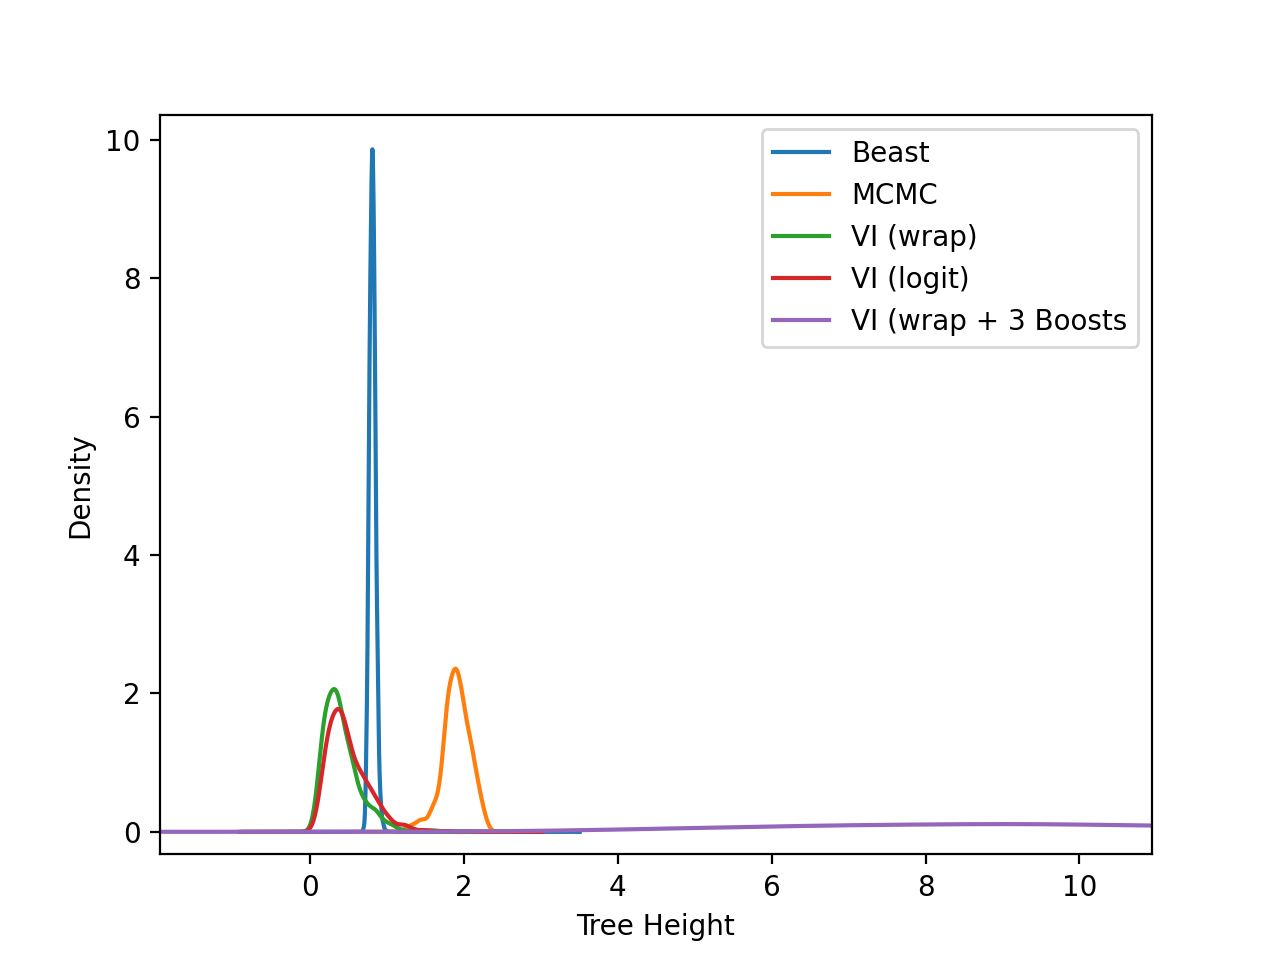
\includegraphics[width=.333\linewidth]{fig/cmp_height}%
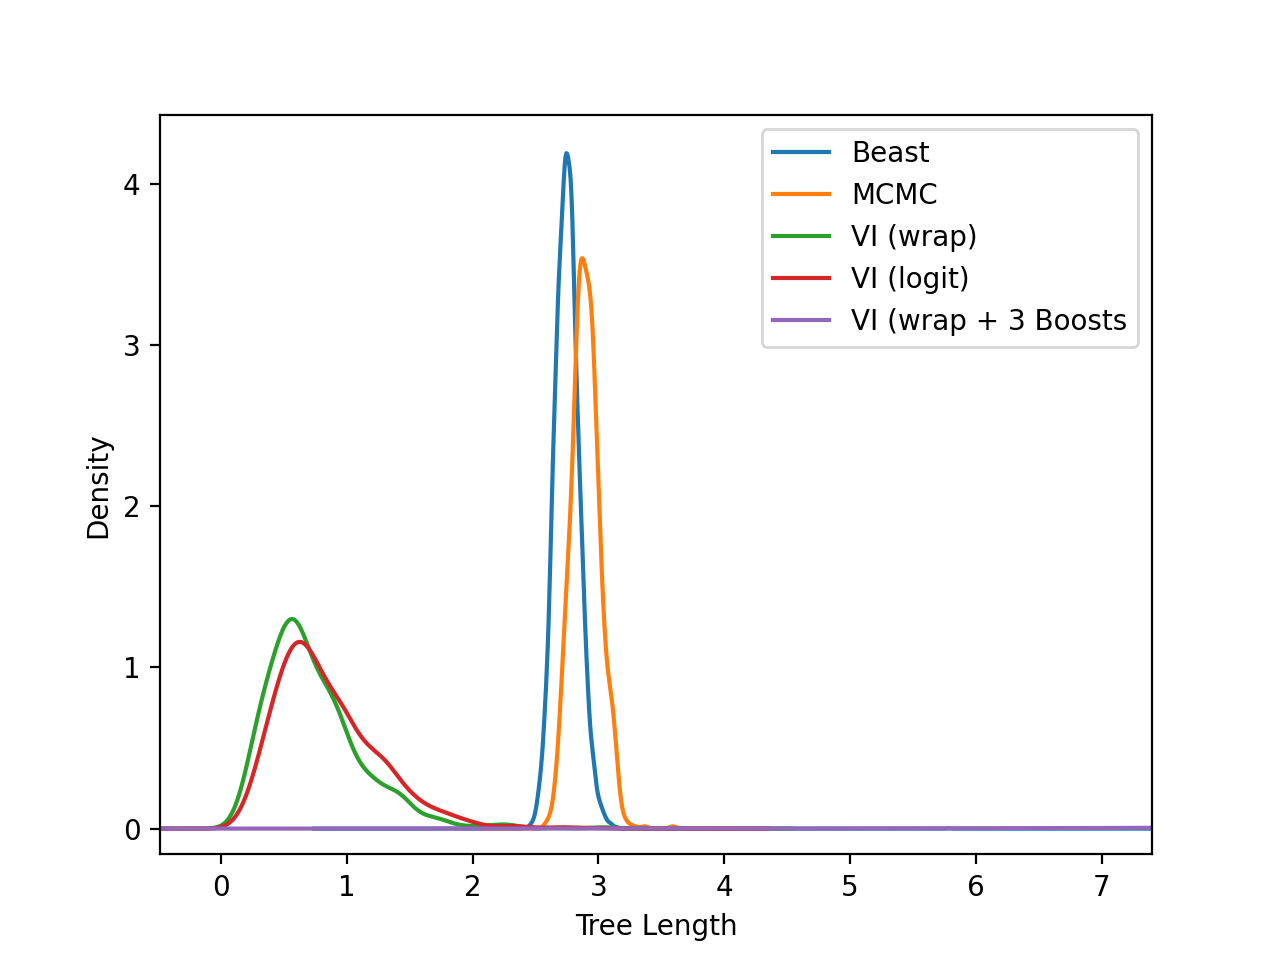
\includegraphics[width=.333\linewidth]{fig/cmp_length}%
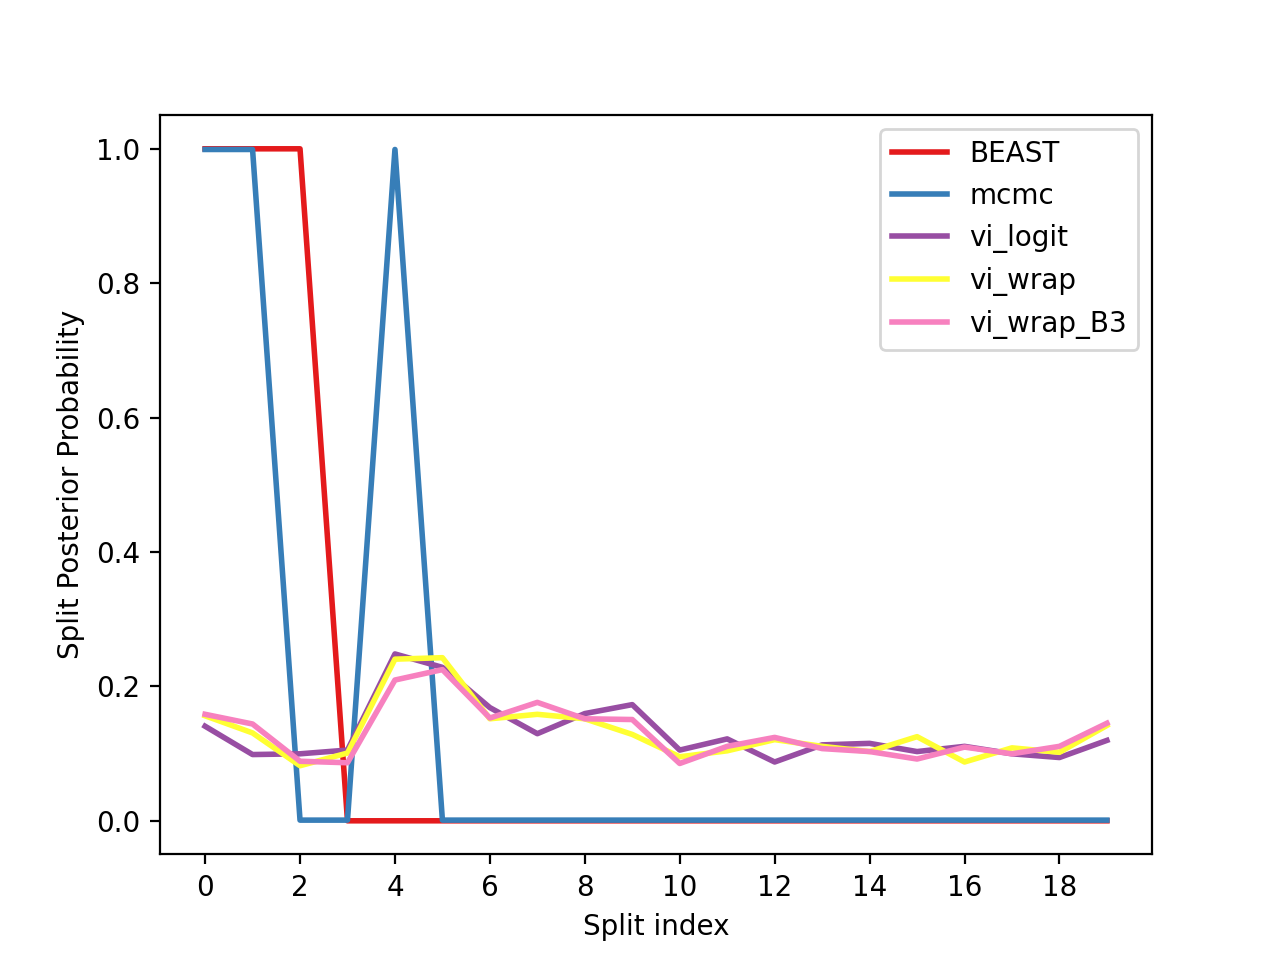
\includegraphics[width=.333\linewidth]{fig/cmp_splits}
\caption{Comparison of tree statistics between Beast and Dodonaphy. Analysis of the splits reveals that BEAST always recovered the simulated tree, whilst our MCMC got 2 splits correct but incorrectly split $16|2345$ instead of $36|245$.}
\label{fig:stat_cmp}
\end{center}
\end{figure}


\section{Variational Inference}
The posterior surface of each node in $\mathbb{H}^{n}$ is unlikely to be continuous (let alone differentiable) as a node changes from one topology to another. But in VI, we don't get a point estimate of the surface, we sample $k$ times from nearby, as if the surface were coarse grained.

\begin{itemize}
\item Are the embedding locations from MCMC normally distributed?
\item What is we learn the curvature?
\item Effect of $k_{samples}$, boosts, learning rate?
\item How easy is it to add taxa? Might only need pair-wise distance to a subset of other taxa.
\item How close is the elbo to known methods?
\end{itemize}

As a toy example, a posterior was generated for a six taxa set using Dodonaphy's MCMC and its VI before being compared to a BEAST MCMC. The data were simulated using a birth (rate$2$) death (rate $.5$) model. The final log likelihood from BEAST was -6280 (similar to it's log posterior of -6271). Running Dodonaphy MCMC gave -6280, which is a close match. Figure~\ref{fig:locations} shows a kernel density estimate for each node location at various stages. Comparing figures~\ref{fig:mcmc_locations}a and b reveals that the posterior surface of nodes can drift over the simulation. Is this a problem for MCMC? Well, it should not affect the tree samples, however the posterior surface is not necessarily static over the entire simulation. So figure~\ref{fig:locations} doesn't really reflect a static embedding of the posterior likelihood.

\begin{figure}[htbp]
\begin{center}
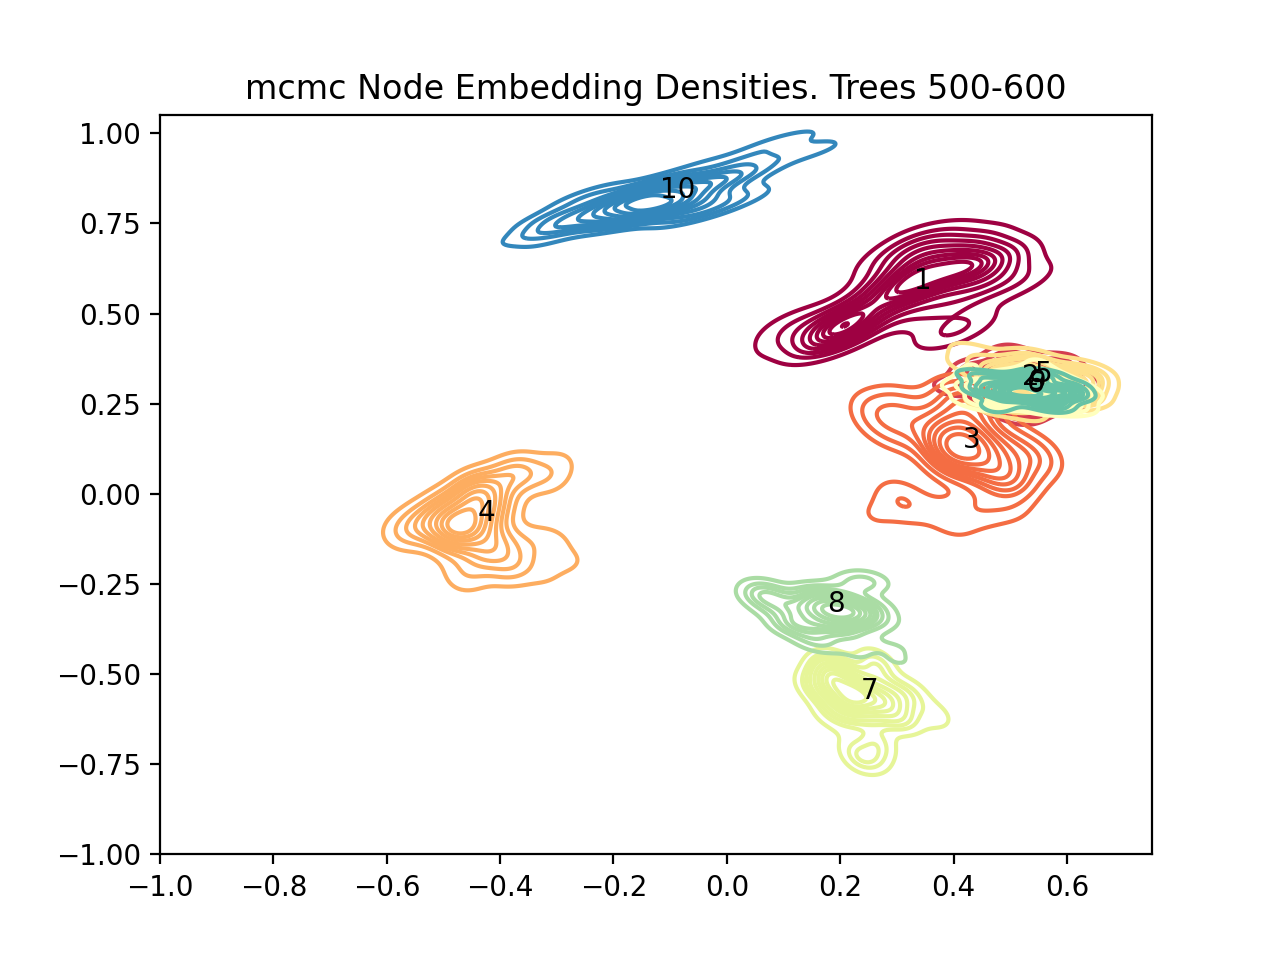
\includegraphics[width=.5\linewidth]{fig/locations_500.png}%
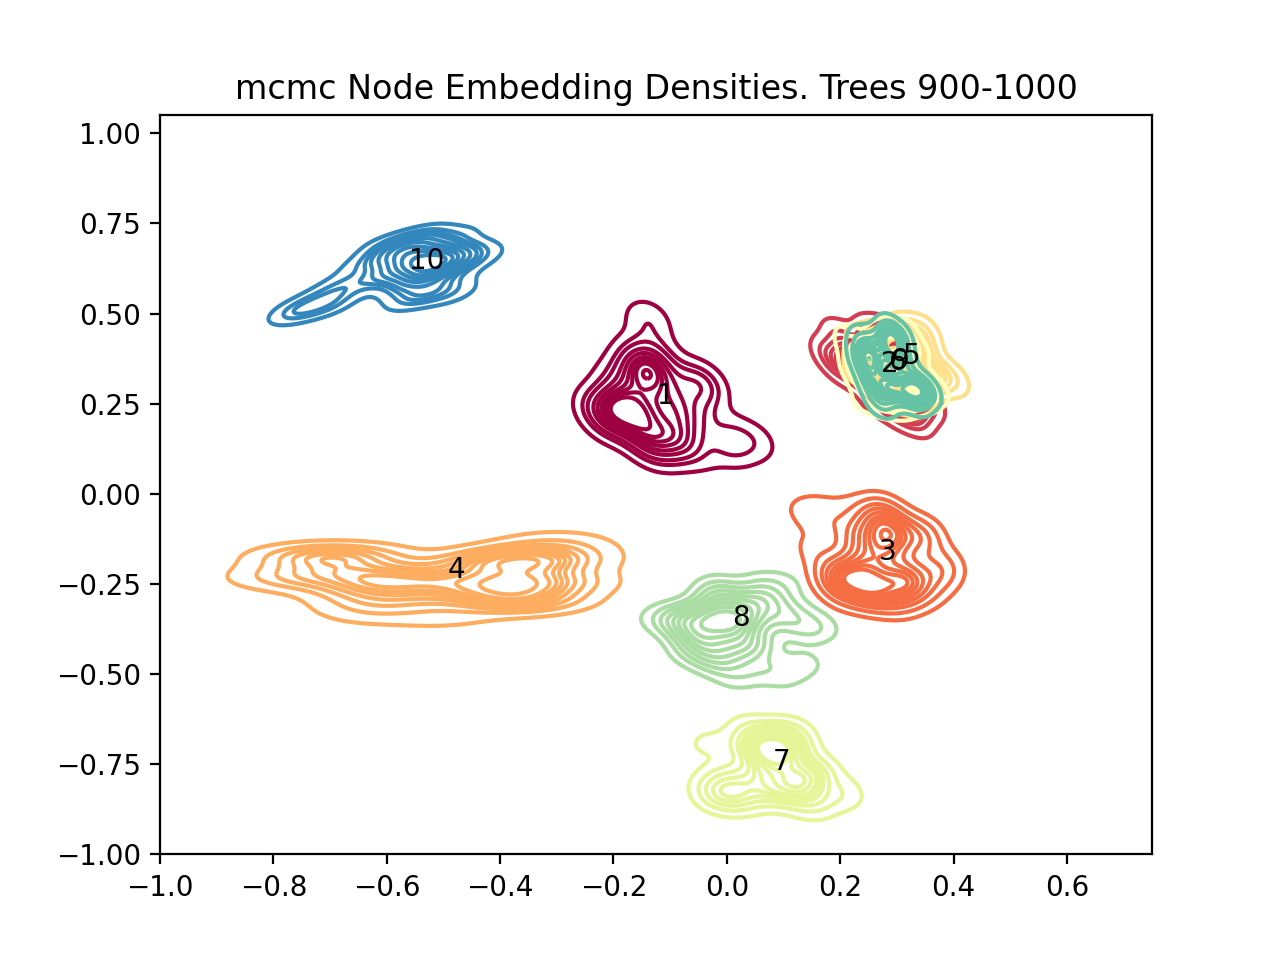
\includegraphics[width=.5\linewidth]{fig/locations_900.png}
\caption{Density estimates of the node locations from Dodonaphy's MCMC projected into $\mathbb{R}^{2}$. (a) Tree 500-600 and (b) 900-1000 in the sampled MCMC chain.}
\label{fig:locations}
\end{center}
\end{figure}

\begin{figure}[htbp]
\begin{center}
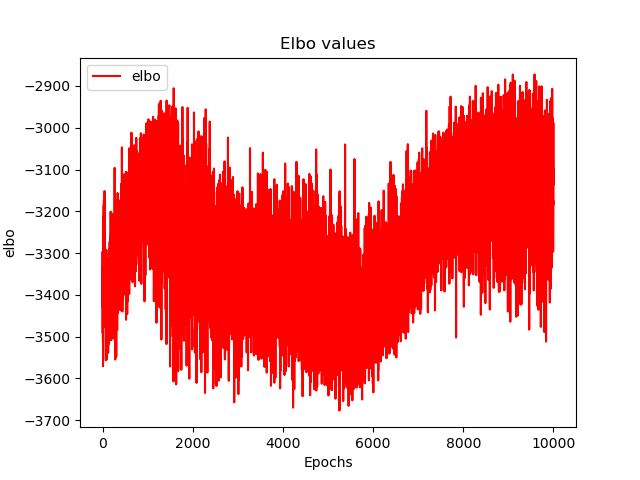
\includegraphics[width=.333\linewidth]{fig/elbo_trace_logit.png}%
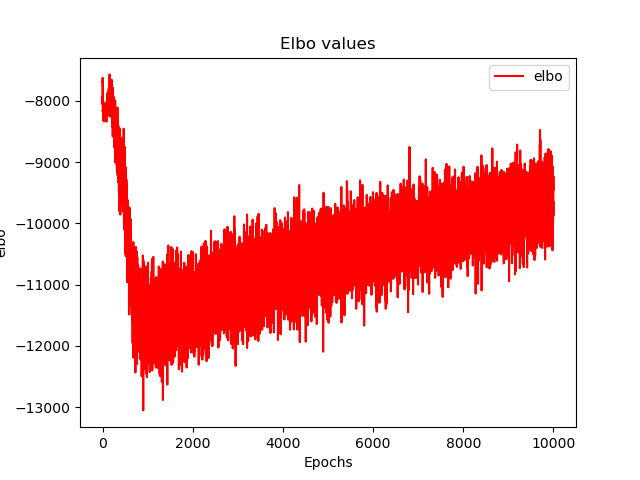
\includegraphics[width=.333\linewidth]{fig/elbo_trace_wrap.png}%
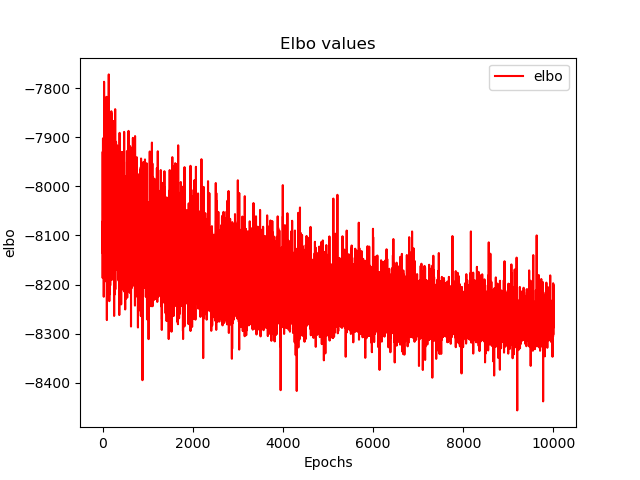
\includegraphics[width=.333\linewidth]{fig/elbo_trace_wrap_B3.png}
\caption{ELBO trace from VI on six taxa using (a) the logit method, (b) the wrapping method and (c) the wrapping method using a mixture of three Gaussians. Simulation used $10^{4}$ epochs, $n=2$ dimensions and $k=10$ samples to evaluate the elbo. Final ELBOs were (a) $-9539$, (b) $-9690$ and (c) -8264.}
\label{fig:elbo}
\end{center}
\end{figure}

\subsection{Initialisation}

\subsection{Full rank}
Intuitively, nodes that are close together should be a bit correlated. However, it doesn't seem to improve things much. In the off-diagonals in the covariance matrix are initialised to zero, the ELBO gets much higher faster compared to if the off-diagonal terms have a non-zero covariance. That said, I haven't run simulations long enough to be sure, only $1000$ epochs with a small learning rate of $0.01$.

\section{Future Thoughts}
Could we adopt an approach like Wilson and Chami, where only the distributions of the embedded points are optimised based on their pair-wise distances.
Only then do we infer a tree.
The advantage of this is that the cost function is differentiable and more in line with what other people in the ML community do.
However, this isn't actually modelling the Bayesian Posterior, just a proxy for it.

We could use boosting (a mixture model).
If we want something more complex, we could introduce a normalizing flows.
I started using the code from ``Variational Inference with Normalizing Flows'' arXiv:1505.05770v6, but didn't get very far.

Since we're doing VI, we needn't really need to embed the distribution of our choosing (Normal) from $\mathbb{R}^{n}$ into $\mathbb{P}^{n}$.
We could instead simply use the original parameterisation with the radius in $r \sim P(N(\mu, \sigma))$ a logit-normal distribution and the directional similarly in a $n$-dimensional logit-normal.



\end{document}  